%%%%%%%%%%%%%%%%%%%%%%%%%%%%%%%%%%%%%%%%%%%%%%%%%%%%%%%%%%%%%%%%%%%%%%
% Lớp 11 | Đường thẳng, mặt phẳng. Quan hệ song song trong | Điểm, đường thẳng và mặt phẳng
% Dạng 1H4?1-6: Ba điểm thẳng hàng, ba đường thẳng đồng quy
% Số câu: 21  (sinh tự động bởi tach_cau.py; từ nay thầy sửa trực tiếp file này)
%%%%%%%%%%%%%%%%%%%%%%%%%%%%%%%%%%%%%%%%%%%%%%%%%%%%%%%%%%%%%%%%%%%%%%

%%%%%%%%%%%%%%%% TRẮC NGHIỆM 4 PHƯƠNG ÁN %%%%%%%%%%%%%%%%

% nguồn: Ok_Toan11_TracNghiem_Lan2
\begin{ex}%[1H4H1-6]%[ma:7f9d99a9]
	 Cho hình chóp $S.ABCD$. Một mặt phẳng $(P)$ bất kỳ cắt các cạnh $SA$, $SB$, $SC$, $SD$ lần lượt tại $A'$, $B'$, $C'$, $D'$. Gọi $I$ là giao điểm của $AC$ và $BD$. Chọn khẳng định đúng trong các khẳng định dưới đây:
	\choice 
		{Các đường thẳng  $AB$, $CD$, $C'D'$ đồng quy}
		{Các đường thẳng $AB$,  $CD$, $A'B'$ đồng quy}
		{\True Các đường thẳng $A'C'$, $B'D'$, $SI$  đồng quy}
		{Các đường thẳng $SB$, $AD$, $B'C'$ đồng  quy}
	 \loigiai{
	\immini{ 
		Hai mặt phẳng $(P)$ và  $(SAC)$ cắt nhau theo giao tuyến $A'C'$.\\
		Hai mặt phẳng $(P)$ và $(SBD)$  cắt nhau theo giao tuyến $B'D'$.\\
		Hai mặt phẳng $(SAC)$  và $(SBD)$ cắt nhau theo giao tuyến $SI$.\\
		Vậy ba đường thẳng $A'C'$,  $B'D'$, $SI$ đồng quy.
		 }{
		\begin{tikzpicture}[>=stealth,line join=round,line cap=round,font=\footnotesize,scale=.8]
				\tikzset{ 
					 pics/hinhChopTuGiacthuong/.style n args={5}{
					 code={
				\tikzset{ 
					 declare function={a=4; b=2; h=3; goc=-130; goc2=-40; c=3.5;}
				 }
				\path 
					(0,0) coordinate (#1)+(0:a) coordinate (#2)+(goc:b) coordinate  (#4)+(80:h) coordinate (#5)+(goc2:c) coordinate (#3);
				 }
					 }}
				\path 
					(0,0) pic  {hinhChopTuGiacthuong={A}{B}{C}{D}{S}}
					(intersection of A--C and B--D)  coordinate (I)
					 ($(S)!.5!(A)$) coordinate (A')
					($(S)!.6!(D)$)  coordinate (D')
					($(S)!.5!(C)$) coordinate (C') 
					(intersection  of A'--C' and S--I) coordinate (I1)
					(intersection of D'--I1 and  S--B) coordinate (B');
				\foreach \pointo/\pointt  in {S/B,S/C,S/D,B/C,C/D,B'/C',C'/D'}{
					\draw[fill=black](\pointo)--(\pointt); 
				 }
				 \foreach \pointo/\pointt in {S/A,A/B,A/D,A/C,B/D,S/I,A'/B',A'/D',A'/C',B'/D'}{
					\draw[fill=black,dashed](\pointo)--(\pointt); 
				 }
				\foreach \point/\goc in {S/90,A/150,B/10,C/-20,D/190,I/-90,A'/130,B'/45,C'/-25,D'/180}{ 
					 \draw[fill=black](\point) circle (.8pt)+(\goc:2mm) node[scale=.8]{$\point$};
				} 
			\end{tikzpicture}
		 }
	} 
\end{ex}

% nguồn: Ok_Toan11_TracNghiem_Lan2
\begin{ex}%[1H4H1-6]%[ma:b568c5f9]
	Cho tứ diện $ABCD$. Gọi $E$, $F$ lần lượt là trung điểm của cạnh  $AB$, $BC$. Mặt phẳng $(P)$ đi qua $EF$ cắt $AD$, $CD$ lần lượt tại $H$ và $G$. Biết $EH$ cắt $FG$ tại $I$. Ba điểm nào sau đây thẳng hàng?
	 \choice
		{$I$,  $A$, $B$}
		 {$I$, $C$, $B$}
		{\True  $I$, $D$, $B$}
		 {$I$, $C$, $D$}
	 \loigiai{
	 \immini{
		Ta có $I = EH  \cap FG$.\\
		 Do đó $\heva{
		&  I \in EH \subset (ABD), \\
		& I  \in FG \subset (ABC)
		} 
		\Rightarrow I \in (ABD) \cap (ABC) = BD$.\\ 
		Vậy $I$, $D$,  $B$ thẳng hàng.
		}{ 
		\begin{tikzpicture}[>=stealth,line join=round,line cap=round,font=\footnotesize,scale=1]
				\tikzset{ 
					pics/chopTamGiac/.style n args={4}{ 
					code={ 
				\tikzset{declare function={a=4; b=3; h=3; goc=-20;}} 
				 \path
					(0,0) coordinate (#1)+(0:a) coordinate (#3)+ 
					(goc:b) coordinate (#2)+(70:h)  coordinate (#4);
				} 
					 }}
				\path 
					(0,0) coordinate (a) pic{chopTamGiac={B}{C}{D}{A}} 
					($(A)!.2!(D)$) coordinate (H) 
					($(A)!.5!(B)$)  coordinate (E)
					($(C)!.2!(D)$) coordinate (G) 
					 (intersection of B--D and H--E) coordinate (I)
					(intersection of G--I and B--C)  coordinate (F);
				\foreach \pointo/\pointt in {A/E,A/C,A/D,H/G,D/C,C/F,F/E,E/I,I/F}{ 
					 \draw[fill=black](\pointo)--(\pointt);
				} 
				\foreach \pointo/\pointt in  {E/B,B/I,B/D,H/E,G/F,F/B}{
					\draw[fill=black,dashed](\pointo)--(\pointt); 
				 }
				\foreach \point/\goc in {D/-20,A/135,B/130,C/-60,I/190,E/150,F/-150,H/60,G/-30}{ 
					\draw[fill=black](\point) circle  (.8pt)+(\goc:2mm) node[scale=.8]{$\point$};
				} 
			\end{tikzpicture}
		} 
	} 
\end{ex}

% nguồn: Ok_Toan11_TracNghiem_Lan2
\begin{ex}%[1H4H1-6]%[ma:4f5a4c70]
	Cho hình chóp tứ giác $S.ABCD$, có đáy $ABCD$ là tứ giác lồi. $O$ là giao  điểm của hai đường chéo $AC$ và $BD$. Một mặt phẳng $(\alpha)$ cắt các cạnh bên $SA$, $SB$, $SC$, $SD$ tương ứng tại các điểm $M$, $N$, $P$, $Q$. Khẳng định nào sau đây đúng?
	\choice 
		{\True Các đường thẳng $MP$, $NQ$, $SO$ đồng quy} 
		{Các đường thẳng $MP$, $NQ$, $SO$  chéo nhau}
		{Các đường thẳng  $MP$, $NQ$, $SO$ đôi một song song}
		{Các đường thẳng $MP$,  $NQ$, $SO$ trùng nhau}
	\loigiai{ 
	\immini{ 
		Ta có $M$, $N$, $P$, $Q$ đồng phẳng và tạo thành tứ giác $MNPQ$ nên hai đường $MP$ và $NQ$  cắt nhau.\\
		Mặt  khác:
		 \[
		 \heva{
		& (MNPQ) \cap (SAC) =  MP, \\
		& (MNPQ) \cap (SBD) = NQ, \\ 
		& (SAC) \cap (SBD) = SO. 
		 }
		\] 
		Từ  đó, suy ra các đường thẳng $MP$, $NQ$, $SO$ đồng quy.
		}{ 
		\begin{tikzpicture}[>=stealth,line join=round,line cap=round,font=\footnotesize,scale=1]
				\tikzset{ 
					pics/hinhChopTuGiacthuong/.style  n args={5}{
					 code={
				 \tikzset{
					 declare function={a=4; b=2; h=3; goc=-130; goc2=-40; c=3.5;}
				} 
				 \path
					(0,0)  coordinate (#1)+(0:a) coordinate (#2)+(goc:b) coordinate (#4)+(80:h) coordinate (#5)+(goc2:c) coordinate (#3);
				} 
					 }}
				 \path
					(0,0) pic {hinhChopTuGiacthuong={A}{B}{C}{D}{S}} 
					(intersection of A--C and B--D) coordinate (O) 
					($(S)!.5!(A)$) coordinate  (M)
					($(S)!.6!(D)$) coordinate  (Q)
					($(S)!.5!(C)$) coordinate (P) 
					(intersection of M--P and  S--O) coordinate (I)
					(intersection of Q--I and S--B)  coordinate (N);
				\foreach  \pointo/\pointt in {S/B,S/C,S/D,B/C,C/D,N/P,P/Q}{
					\draw[fill=black](\pointo)--(\pointt); 
				 }
				\foreach \pointo/\pointt in {S/A,A/B,A/D,A/C,B/D,M/N,M/Q,M/P,N/Q,S/O}{ 
					\draw[fill=black,dashed](\pointo)--(\pointt); 
				 }
				\foreach \point/\goc in {S/90,A/150,B/10,C/-20,D/190,O/-90,M/130,N/45,P/-25,Q/180}{ 
					 \draw[fill=black](\point) circle (.8pt)+(\goc:2mm) node[scale=.8]{$\point$};
				} 
			\end{tikzpicture}
		} 
	} 
\end{ex}

% nguồn: Ok_Toan11_TracNghiem_Lan2
\begin{ex}%[1H4H1-6]%[ma:88a84d32]
	Cho hình tứ diện $ABCD$ có $M$, $N$ lần lượt là trung  điểm của $AB$, $BD$. Các điểm $G$, $H$ lần lượt trên cạnh $AC$, $CD$ sao cho $NH$ cắt $MG$ tại $I$. Khẳng định nào sau đây là khẳng định đúng?
	 \choice
		{$A$, $C$, $I$ thẳng  hàng}
		{\True $B$, $C$, $I$  thẳng hàng}
		{$N$, $G$, $H$  thẳng hàng}
		{$B$, $G$, $H$  thẳng hàng}
	 \loigiai{
		\begin{center}
			\begin{tikzpicture}[scale=1,font=\footnotesize,line join=round,line cap=round,>=stealth]
					 \path
						(0,0) coordinate (B) 
						(1,-2)  coordinate (C)
						(4,0) coordinate  (D)
						(1.5,3.4) coordinate (A) 
						 ($(A)!0.5!(B)$) coordinate (M)
						 ($(B)!.5!(D)$) coordinate (N)
						($(A)!2/3!(C)$) coordinate (G) 
						($(D)!2/3!(C)$) coordinate  (H)
						(intersection of N--H and  M--G) coordinate (I);
					\draw (D)--(A)--(B)--(C)--(I) 
						 (H)--(D)
						 (A)--(C)
						 (H)--(I)
						 (M)--(I);
					\draw[dashed] (B)--(D) 
						 (M)--(N)--(H)--(C);
					\foreach \p/\q in {A/90,B/180,C/-120,D/0,M/140,N/30,I/-90,G/0,H/-30} 
					 \fill (\p) circle (1.0pt)
						 ($(\p)+(\q:2.5mm)$) node{$\p$};
				\end{tikzpicture}
		\end{center}
		Do $NH$ cắt $MG$ tại $I$ nên bốn điểm $M$, $N$, $H$, $G$  cùng thuộc mặt phẳng $(\alpha)$.\\
		 Ta có $\heva{&(\alpha) \cap(ABC)=MG\\
		&(\alpha) \cap(BCD)=NH\\ 
		 &(ABC) \cap(BCD)=BC}$ mà $MG\cap NH=I$.\\
	 Suy ra $MG$, $NH$, $BC$ đồng quy tại $I$ nên $B$, $C$, $I$ thẳng hàng}
\end{ex}

% nguồn: Ok_Toan11_TracNghiem_Lan2
\begin{ex}%[1H4H1-6]%[ma:b16f2d53]
	Cho hình chóp $S.ABCD$ có đáy là hình thang $ABCD$ ($AD \parallel BC$, $AD > BC$). Gọi $I$ là  giao điểm của $AB$ và $DC$; $M$ là trung điểm của $SC$ và $M$ cắt mặt phẳng $(SAB)$ tại $J$. Khẳng định nào sau đây \textbf{sai}?
	 \choice
		{Đường thẳng $SI$ là giao tuyến của hai mặt phẳng $(SAB)$ và  $(SCD)$}
		{\True Đường thẳng $JM$ thuộc mặt phẳng $(SAB)$} 
		{Ba điểm $S$, $I$,  $J$ thẳng hàng}
		{ Đường thẳng $DM$  thuộc mặt phẳng $(SCI)$}
	\loigiai{ 
	 \immini{
		Ta có  $M \notin (SAB)$ nên đường thẳng $JM$ không thuộc mặt phẳng $(SAB)$.
		 }{
		\begin{tikzpicture}[>=stealth,line join=round,line cap=round,font=\footnotesize,scale=1]
				\tikzset{ 
					 pics/hinhChopTuGiacHinhThang/.style n args={5}{
					code={ 
				 \tikzset{
					 declare function={a=2.5; b=1.2; h=2.5; goc=-60;}
				} 
				\path 
					 (0,0) coordinate (#1)+(0:a) coordinate (#2)+(goc:b) coordinate (#4)+(60:h) coordinate (#5)
					 ($(#2)+(#4)-(#1)$) coordinate (c)
					($(c)!.5!(#4)$)  coordinate (#3);
				} 
					 }}
				\path 
					 (0,0) pic {hinhChopTuGiacHinhThang={A}{D}{C}{B}{S}}
					(intersection  of A--B and C--D) coordinate (I)
					($(S)!.5!(C)$) coordinate  (M)
					(intersection of S--I and D--M)  coordinate (J);
				\foreach \pointo/\pointt in  {S/B,S/C,S/D,S/A,A/B,C/D,B/I,C/I,S/I,J/D}{
					 \draw[fill=black](\pointo)--(\pointt);
				 }
				\foreach \pointo/\pointt in  {A/D,B/C}{
					\draw[fill=black,dashed](\pointo)--(\pointt); 
				} 
				\foreach \point/\goc  in {A/190,S/90,B/190,C/-20,D/-10,I/-90,M/45,J/60}{
					 \draw[fill=black](\point) circle (.8pt)+(\goc:2mm) node[scale=.8]{$\point$};
				} 
			\end{tikzpicture}
		 }
	} 
\end{ex}

% nguồn: Ok_Toan11_TracNghiem_Lan2
\begin{ex}%[1H4H1-6]%[ma:80f78595]
	Cho hình chóp tứ giác $S.ABCD$, gọi $O$ là giao điểm của $AC$ và $BD$. Một mặt phẳng $(\alpha)$ cắt các cạnh bên $SA$, $SB$, $SC$, $SD$ tương ứng tại các điểm $M$,  $N$, $P$, $Q$. Khẳng định nào đúng?
	 \choice
		{Các đường  thẳng $MN$, $PQ$, $SO$ đồng quy}
		{\True Các đường thẳng $MP$, $NQ$, $SO$ đồng quy} 
		{Các đường thẳng  $MQ$, $PN$, $SO$ đồng quy}
		{Các  đường thẳng $MQ$, $PQ$, $SO$ đồng quy}
	\loigiai{ 
	 \immini{
		Ta  có $
		\heva{ 
		&  MP \subset (SAC) \\
		&  NQ \subset (SBD) \\
		& (SAC) \cap (SBD) =  SO.
		}$\\ 
		Gọi $I = MP \cap NQ$ thì $I \in SO$, nên các đường thẳng $MP$, $NQ$,  $SO$ đồng quy.
		 }{
		\begin{tikzpicture}[>=stealth,line join=round,line cap=round,font=\footnotesize,scale=1]
				\tikzset{ 
					 pics/hinhChopTuGiacthuong/.style n args={5}{
					 code={
				 \tikzset{
					declare function={a=4;  b=2; h=3; goc=-150; goc2=-40; c=3.5;}
				} 
				 \path
					(0,0) coordinate (#1)+(0:a)  coordinate (#2)+(goc:b) coordinate (#4)+(80:h) coordinate (#5)+(goc2:c) coordinate (#3);
				 }
					 }}
				 \path
					(0,0)  pic {hinhChopTuGiacthuong={B}{C}{D}{A}{S}}
					(intersection of A--C and B--D) coordinate (O) 
					($(S)!.45!(A)$) coordinate  (M)
					($(S)!.55!(D)$) coordinate  (Q)
					($(S)!.45!(C)$)  coordinate (P)
					(intersection of M--P  and S--O) coordinate (I)
					(intersection of  Q--I and S--B) coordinate (N);
				\foreach  \pointo/\pointt in {S/A,S/D,S/C,C/D,D/A,M/Q,Q/P}{
					 \draw[fill=black](\pointo)--(\pointt);
				 }
				 \foreach \pointo/\pointt in {S/B,B/A,A/C,C/B,B/D,S/O,N/M,N/P,M/P,N/Q}{
					 \draw[fill=black,dashed](\pointo)--(\pointt);
				 }
				\foreach  \point/\goc in {S/90,A/190,B/150,C/-20,D/-90,O/-90,M/190,N/145,P/25,Q/-30}{
					\draw[fill=black](\point) circle (.8pt)+(\goc:2mm)  node[scale=.8]{$\point$};
				 }
			\end{tikzpicture}
		 }
	 }
\end{ex}

% nguồn: Ok_Toan11_TracNghiem_Lan2
\begin{ex}%[1H4H1-6]%[ma:9a25d868]
	Cho tứ diện $ABCD$. Gọi $M$, $N$ lần lượt là trung điểm $AB$ và $CD$. Mặt phẳng $(\alpha)$ qua $MN$ cắt $AD$  và $BC$ lần lượt tại $P$, $Q$. Biết $MP$ cắt $NQ$ tại $I$. Ba điểm nào sau đây thẳng hàng?
	 \choice
		 {$I$, $A$, $C$}
		{\True  $I$, $B$, $D$}
		{$I$,  $A$, $B$}
		{$I$, $C$,  $D$}
	\loigiai{ 
		\begin{center}
			\begin{tikzpicture}[scale=1,font=\footnotesize,line join=round,line cap=round,>=stealth]
					 \path
						 (0,0) coordinate (B)
						(1.5,-2) coordinate (C) 
						 (4,0) coordinate (D)
						(2,3) coordinate (A) 
						($(A)!0.5!(B)$)  coordinate (M)
						($(D)!.5!(C)$) coordinate (N) 
						 ($(B)!1/3!(C)$) coordinate (Q)
						 (intersection of N--Q and B--D) coordinate (I)
						(intersection of  I--M and A--D) coordinate (P);
					\draw  (I)--(M)--(A)--(D)--(C)--(Q)--cycle
						 (A)--(C)
						(N)--(P) 
						 (Q)--(M);
					 \draw[dashed] (I)--(D)
						 (P)--(I)--(N)
						 (C)--(B)--(A);
					\foreach  \p/\q in {A/90,B/135,C/-90,D/40,M/115,N/-30,P/0,Q/210,I/180}
					\fill  (\p) circle (1.0pt)
						($(\p)+(\q:2.5mm)$)  node{$\p$};
				\end{tikzpicture}
		\end{center}
		Ta  có $\heva{&(\alpha)\cap (ABD)=MP\\&(\alpha)\cap (BCD)=NQ\\&(BCD)\cap (ABD)=BD}.$\\
		Mà $I=MP\cap NQ$ nên $I\in BD$ hay $B$, $I$, $D$  thẳng hàng.
	} 
\end{ex}

% nguồn: Ok_Toan11_TracNghiem_Lan2
\begin{ex}%[1H4H1-6]%[ma:7b2538fb]
	Cho tứ diện $SABC$. Gọi $L$, $M$, $N$  lần lượt là các điểm trên các cạnh $SA$, $SB$, $AC$ sao cho $LM$ không song song $AB$, $LN$ không song song $SC$. Mặt phẳng $(LMN)$ cắt các cạnh $AB$, $BC$, $SC$ lần lượt tại $K$, $I$, $J$. Ba điểm nào sau đây thẳng hàng?
	\choice 
		 {$A$, $I$, $J$}
		{$S$, $I$,  $J$}
		{\True $M$,  $I$, $J$}
		 {$L$, $I$, $J$}
	\loigiai{ 
		\begin{center}
			\begin{tikzpicture}[scale=1,font=\footnotesize,line join=round,line cap=round,>=stealth]
					\path 
						(0,0) coordinate  (A)
						 (1.5,-2) coordinate (B)
						(5,0) coordinate (C) 
						 (2,3) coordinate (S)
						($(S)!2/3!(B)$) coordinate  (M)
						($(A)!4/5!(C)$)  coordinate (N)
						 ($(S)!2/5!(A)$) coordinate (L)
						(intersection  of L--M and A--B) coordinate (K)
						 (intersection of N--K and C--B) coordinate (I)
						(intersection of N--L and  C--S) coordinate (J)
						(intersection of N--L and  C--B) coordinate (N1);
					\draw (S)--(A)--(B)--(K)--(I)--(C)--(S)--(B) 
						 (L)--(K)
						 (C)--(J)--(N1);
					\draw[dashed] (C)--(A) 
						 (L)--(N)--(I)--(B)
						(N)--(N1); 
					\foreach  \p/\q in {A/180,B/-120,C/0,S/90,M/45,N/30,L/180,K/-90,I/0,J/0}
					\fill  (\p) circle (1.0pt)
						($(\p)+(\q:2.5mm)$) node{$\p$}; 
				\end{tikzpicture}
		\end{center}
		Ta có $K=(LMN)\cap AB$; $I=(LMN)\cap  BC$; $J=(LMN)\cap SC$.\\
		Suy ra $\heva{&I\in BC\subset (SBC)\\&I\in (LMN)}\Rightarrow I\in (SBC)\cap  (LMN)$.\\
		 Ta lại có $\heva{&J\in SC\subset (SBC)\\&J\in (LMN)}\Rightarrow J\in (SBC)\cap (LMN)$.\\
		Mặt khác $\heva{&M\in SB\subset (SBC)\\&M\in (LMN)}\Rightarrow  M\in (SBC)\cap (LMN)$.\\
		Từ đó suy ra ba điểm  $M$, $I$, $J$ cùng thuộc hai $(LMN)$ và $(SBC)$.\\
		Vậy ba điểm $M$, $I$, $J$ thẳng hàng do cùng nằm trên giao tuyến của hai mặt phẳng $(LMN)$  và $(SBC)$.
	} 
\end{ex}


%%%%%%%%%%%%%%%% ĐÚNG/SAI %%%%%%%%%%%%%%%%

% nguồn: Ok_dungsai_lop11_Lan1
\begin{ex}%[1H4H1-6]%[ma:8cce2d99]
 Cho hình chóp $S.ABCD$ có đáy $ABCD$ là hình thang ( $AD$ là đáy lớn, $BC$ là đáy nhỏ). Gọi $E$, $F$ lần lượt là trung điểm của $SA$ và $SD$ với $K$ là giao điểm của các  đường thẳng $AB$ và $CD$. Khi đó
  \choiceTF
  {\True Giao điểm $M$ của đường thẳng $SB$ và mặt  phẳng $(CDE)$ là điểm thuộc đường thẳng $KE$}
  {Đường thẳng $SC$  cắt mặt phẳng $(EFM)$ tại $N$. Tứ giác $EFNM$ là hình bình hành}
  {\True Các đường thẳng $AM$, $DN$, $SK$  cùng đi qua một điểm}
  {\True Cho biết $AD=2BC$. Tỉ số diện tích của hai tam giác $KMN$ và $KEF$ bằng  $\dfrac{S_{\triangle KMN}}{S_{\triangle KEF}}=\dfrac{2}{3}$}
 \loigiai{\begin{center}
  \begin{tikzpicture}[line join=round,line cap=round,>=stealth,thick]
     \coordinate (A) at (-2,0);
    \coordinate (B)  at (-1,-1.4);
     \coordinate (C) at (1,-1.4);
    \coordinate (D) at  (2,0);
     \coordinate (S) at (0.4,4);
    \coordinate (K) at  (0,-2.8);
    \coordinate (E)  at ($(S)!0.5!(A)$);
    \coordinate (F) at  ($(S)!0.5!(D)$);
    \coordinate (I) at  ($(S)!0.5!(K)$);
    \draw  (S)--(A)
     (A)--(K) 
     (K)--(D) 
      (S)--(K)
      (S)--(D)
      (S)--(B)
      (K)--(E)
      (A)--(I)
     (I)--(D) 
     (S)--(C) 
     (K)--(F); 
    \coordinate (M) at (intersection  of K--E and S--B);
     \coordinate (N) at (intersection of K--F and I--D);
    \draw[dashed](A)--(D) 
     (B)--(C) 
      (E)--(F)
     (C)--(E) 
     (D)--(E) 
     (M)--(N); 
    \foreach \i in  {S,A,B,C,D,M,N,I,E,F,K}{\draw[fill=](\i) circle (1pt);}
    \foreach \i  in {S}{\draw (\i) node[scale=0.9,above]{$\i$};}
    \foreach  \i in {E,A,B}{\draw (\i) node[scale=0.9,left]{$\i$};}
    \foreach \i  in {M}{\draw (\i) node[scale=0.9,above left]{$\i$};}
    \foreach \i in {F,D,C,I}{\draw (\i) node[scale=0.9,right]{$\i$};} 
    \foreach \i in {N}{\draw (\i)  node[scale=0.9,above right]{$\i$};}
    \foreach \i in {K}{\draw (\i)  node[scale=0.9,below]{$\i$};}
   \end{tikzpicture}
 \end{center}
 \begin{itemchoice}
  \itemch \textbf{Đúng}. Có $SK=(SAB)  \cap(SCD)$.\\
  Trong mp $(SAB)$, gọi $M=KE \cap SB$, có $KE \subset(CDE)$.\\ Do đó $SB  \cap(CDE)=M$.
  \itemch \textbf{sai}. Trong mp $(SCD)$, gọi $N=KF \cap  SC$, có $KF \subset(EFM)$.\\
   Do đó $SC \cap(EFM)=N$. \\
   $\Rightarrow \heva{&MN=(EFK) \cap(SBC)\\&EF\parallel BC,\, EF \subset(EFK),\, BC \subset(SBC).}$\\
  $\Rightarrow MN \parallel EF  \parallel BC$.\\
  Suy ra tứ  giác $EFNM$ là hình thang.
  \itemch \textbf{Đúng}. Trong  mp $(ADNM)$, gọi $I=AM \cap DN$.\\
  Mà $\heva{&I \in AM,\, AM \subset(SAB) \\ &I \in CD,\, CD \subset(SCD)} \Rightarrow I  \in(SAB) \cap(SCD)$.\\
   Hay $I \in SK$. Kết luận $3$ đường thẳng $AM$, $DN$, $SK$ đồng quy tại điểm $I$.
  \itemch \textbf{Đúng}. Khi $AD=2BC$ nên $B$, $C$ lần lượt là trung điểm của $KA$ và $KD$.\\  Suy ra $M$, $N$ lần lượt là trọng tâm của hai tam giác $SAK$ và $SDK$.\\
  Do đó $MN=\dfrac{2}{3} EF$, gọi $h_1$, $h_2$ lần lượt là độ dài đường cao xuất phát từ đỉnh $K$ xuống hai đáy $MN$ và  $EF$, dễ thấy $h_1=\dfrac{2}{3}h_2$.\\
   Vậy $\dfrac{S_{\triangle KMN}}{S_{\triangle KEF}}=\dfrac{\dfrac{1}{2} MN \cdot h_1}{\dfrac{1}{2} EF \cdot h_2}=\dfrac{\dfrac{2}{3} EF \cdot \dfrac{2}{3}h_2}{EF \cdot h_2}=\dfrac{4}{9}$.
\end{itemchoice} }
\end{ex}

% nguồn: Ok_dungsai_lop11_Lan1
\begin{ex}%[1H4H1-6]%[ma:eaefde06]
 Trong mặt phẳng $(P)$, cho  hình bình hành $ABCD$ tâm $O$, ngoài mặt phẳng $(P)$ cho một điểm $S$.
 \choiceTF 
  {Điểm $C$ là một điểm chung của hai  mặt phẳng $(SAB)$ và $(SCD)$}
  {\True  Giao tuyến của hai mặt phẳng $(SCB)$ và $(SCD)$ là đường thẳng $SC$}
  {\True Giao điểm của mặt phẳng $(SAC)$ với đường thẳng $BD$ là  điểm $O$}
  {Giao điểm của đường thẳng $BC$ với mặt phẳng $(SBD)$ là điểm $C$} 
  \loigiai{
  \begin{center}
   \begin{tikzpicture}[scale=1,font=\footnotesize,line join=round,line cap=round,>=stealth,blue,thick]
     \def\bc{4} 
      \def\ba{2}
      \def\h{4}
      \def\gocB{35}
     \coordinate (M) at  (-1.5,-.5);
     \coordinate (N) at  (50:2.5);
     \coordinate (Q) at  (5,-.5);
      \coordinate (P) at ($(Q)-(M)+(N)$);
      \fill[cyan!20!](M)--(N)--(P)--(Q)--cycle;
     \coordinate[label=below left:$D$]  (D) at (0,0);
      \coordinate[label=above left:$A$] (A) at (\gocB:\ba);
     \coordinate[label=below:$C$] (C)  at (\bc,0);
     \coordinate[label=above right:$B$]  (B) at ($(C)-(D)+(A)$);
      \path
      (intersection  of A--C and B--D) coordinate (O);
      \node at (O) [below]{$O$};
     \coordinate  [label=above:$S$](S) at ($(O)+(0,4)$);
     \draw  (S)--(D)--(C)--(B)--cycle;
     \draw[dashed,thin] (A)--(C)--(S) 
       (B)--(D)
      (A)--(S)--(O) 
      (D)--(A)--(B); 
      \draw pic["$P$",draw=black,angle eccentricity=.7,angle radius=1cm] {angle=Q--M--N};
     \foreach \i in  {A,B,C,D,O,S} \fill[black] (\i) circle (1pt);
    \end{tikzpicture}
  \end{center}
  \begin{itemchoice}
   \itemch Sai. Điểm $C$ không là một điểm chung của  hai mặt phẳng $ (SAB)$ và $(SCD)$ vì điểm $C$ không không thuộc mặt phẳng $(SAB)$
   \itemch Đúng. Vì $S$ và $C$ cùng thuộc hai mặt phẳng $(SCB)$ và $ (SCD)$  nên giao tuyến của hai mặt phẳng $(SCB)$ và $(SCD)$ là đường thẳng $SC$.
   \itemch Đúng. Khi đó vì $O$ thuộc mặt phẳng $(SAC)$ nên điểm $O$ là giao điểm của mặt phẳng $(SAC)$ với đường thẳng  $BD$.
   \itemch Sai. Vì  giao điểm của đường thẳng $BC$ với mặt phẳng $(SBD)$ là điểm $B$.
  \end{itemchoice}
 } 
\end{ex}

% nguồn: Ok_dungsai_lop11_Lan2
\begin{ex}%[1H4H1-6]%[ma:d15544d4]
	Cho hình chóp $S.ABCD$ có đáy  là hình bình hành. Gọi $O$ là giao điểm của $AC$ và $BD$; $M$, $N$ lần lượt là trung điểm của $SB$, $SD$; $P$ thuộc đoạn $SC$ và không là trung điểm của $SC$. Khi đó
	 \choiceTF
		{\True Giao điểm $E$ của đường thẳng $SO$ và mặt phẳng $(MNP)$ là giao  điểm của $PE$ và $SO$}
		{Giao điểm $Q$ đường thẳng $SA$ và mặt phẳng $(MNP)$ là giao điểm của $PE$ và $SO$} 
		{\True Gọi $I$, $J$, $K$ lần lượt là giao điểm của $QM$ và  $AB$,$QP$ và $AC$, $QN$ và $AD$. Vậy $I$, $J$, $K$ thẳng hàng}
		{Gọi $I$, $J$, $K$ lần lượt là giao điểm của $QM$ và $AB$,$QP$  và $AC$, $QN$ và $AD$. Vậy $I$, $J$, $K$ không thẳng hàng}
	\loigiai{ 
		\begin{center}
			\begin{tikzpicture}[scale=.7,font=\footnotesize,line join=round,line cap=round,>=stealth]
					 \path
						(0,0) coordinate (A) 
						(5,0)  coordinate (D)
						(3,-1.5)  coordinate (C)
						(-2,-1.5) coordinate (B) 
						(-0.6,5) coordinate  (S)
						($(A)!0.5!(C)$)  coordinate (O)
						 ($(B)!0.5!(S)$) coordinate (M)
						 ($(D)!0.5!(S)$) coordinate (N)
						 ($(C)!0.35!(S)$) coordinate (P);
					\path [name path =mn] (M)--(N); 
					\path [name  path =so] (S)--(O);
					\path [name intersections ={of  =mn and so,by={E}}];
					\path [name path =sa]  (S)--(A);
					\path  [name path =pq] (E)--($(E)!1!180:(P)$);
					\path [name intersections ={of =sa  and pq,by={Q}}];
					\path [name  path =ai] (B)--($(B)!2.5!180:(A)$);
					\path [name path  =iq] (M)--($(M)!6!180:(Q)$);
					\path [name intersections ={of =iq and  ai,by={I}}];
					\path [name  path =ak] (D)--($(D)!2.3!180:(A)$);
					\path  [name path =kq] (N)--($(N)!5.5!180:(Q)$);
					\path [name intersections ={of =kq and ak,by={K}}]; 
					\path [name path =aj] (C)--($(C)!1!180:(A)$); 
					\path [name path =qj]  (P)--($(P)!2!180:(Q)$);
					\path [name intersections ={of =aj  and qj,by={J}}];
					 \draw (S)--(M)--(I)--(K)--(N)--(S)--(P)--(J)
						 (M)--(P)--(N)--(S)
						(P)--(N); 
					 \draw[dashed] (M)--(B)
						 (N)--(D)
						 (I)--(A)--(K)
						 (B)--(C)--(J)
						 (D)--(C)--(A)
						 (B)--(D)
						(A)--(S)--(O) 
						(M)--(Q)--(N)--(M) 
						(C)--(P)--(Q); 
					 \foreach \i/\g in {A/160,B/-90,C/-90,D/45,S/90,E/-120,I/-135,J/-90,K/0,O/-90,M/160,N/45,Q/150,P/30}
					\fill[black] (\i) circle (1pt)+(\g:3.5mm) node[scale=1]{$\i$}; 
				\end{tikzpicture}
		\end{center}
		\begin{itemchoice}
			\itemch  Trong $(SBD)$ gọi $E= SO\cap MN$.\\
			Ta có  $\heva{&E\in SO\\&E\in MN\subset(MNP)}$ suy ra $E\in SO\cap(MNP)$.
			\itemch Trong  $(SAC)$ gọi $Q=PE\cap SA$.\\
			Ta có $\heva{&Q\in SA\\&Q\in PE\subset(MNP)}$  suy ra $Q\in SA\cap(MNP)$.
			\itemch Từ giả thiết ta có $\heva{&I\in QM\subset(MNP)\\&J\in QP\subset(MNP)\\&K\in QN\subset(MNP)}$ suy ra $I$, $J$, $K\in(MNP)\  (1)$.\\
			Mặt khác $\heva{&I\in AB\subset(ABCD)\\&J\in AC\subset(ABCD)\\&K\in AD\subset(ABCD)}$ suy ra $I$, $J$,  $K\in(ABCD)\ (2)$.\\
			Từ $(1)$ và $(2)$ suy ra $I$, $J$, $K\in(MNP)\cap(ABCD)$. Suy ra $I$, $J$,  $K$ thẳng hàng.
			\itemch Gọi $I$, $J$, $K$ lần  lượt là giao điểm của $QM$ và $AB$, $QP$ và $AC$, $QN$ và $AD$.\\
			Ta  có $\heva{&I\in QM\subset (QMNP)\\&I\in AB\subset ABCD} \Rightarrow I\in (ABCD)\cap (MNPQ).
			 $\\
			$\heva{&J\in QP\subset (QMNP)\\&J\in AC\subset ABCD} \Rightarrow J\in (ABCD)\cap (MNPQ). 
			 $\\
			$\heva{&K\in QN\subset (QMNP)\\&K\in AD\subset  ABCD} \Rightarrow K\in (ABCD)\cap (MNPQ).
			 $\\
			Vậy $I$, $J$, $K$ thẳng hàng. 
		\end{itemchoice}
	 }
\end{ex}


%%%%%%%%%%%%%%%% TRẢ LỜI NGẮN %%%%%%%%%%%%%%%%

% nguồn: Ok_TraLoiNgan_Lop11_Lan1
\begin{ex}%[1H4N1-6]%[ma:a5130de1]
	Cho ba điểm $A$, $B$, $C$ không thẳng hàng và không thuộc mp $(Q)$, các đường thẳng $BC$, $CA$, $AB$ cắt $(Q)$ lần lượt tại $F$, $E$, $D$. Hỏi  ba điểm $D$, $E$, $F$ có thẳng hàng không? có thẳng hàng chọn $1$, không thẳng hàng chọn $2$, trùng nhau chọn $3$, không nằm ở trường hợp nào của các lựa chọn trước thì chọn $4$.
	 \shortans{1}
	\loigiai{ 
	\immini 
		{Ta có $F$, $E$, $D$ lần lượt thuộc hai mặt phẳng $(Q)$ và $(ABC)$ nên $F$,  $E$, $D$ thuộc giao tuyến $d$ của $(Q)$ và $(ABC)$. \\
		Vậy $D$, $E$, $F$ thẳng  hàng.
		 }
		{\begin{tikzpicture}[line join = round,line cap = round,>=stealth,font=\footnotesize,scale=0.7]
		\path (0,0) coordinate (M) 
			+(-2,-2)  coordinate (N)
			+(5,0) coordinate  (P)
			($(N)+(P)-(M)$) coordinate (Q) 
			(3,2) coordinate  (A)
			(2,1) coordinate (B) 
			(2.5,0.5) coordinate  (C)
			(4,-0.5) coordinate  (G);
		\coordinate[label=above:$d$] (H)  at (-0.9,-1.5);
		\draw pic[angle radius=7mm,draw=blue,fill=green!50,opacity=.5,"$Q$",angle eccentricity=.7] {angle  = Q--N--M};
		\coordinate  (D) at (intersection cs:first line={(H)--(G)},second line={(A)--(B)});
		 \coordinate (E) at (intersection cs:first line={(H)--(G)},second line={(A)--(C)});
		\coordinate (F)  at (intersection cs:first line={(H)--(G)},second line={(B)--(C)});
		\draw (H)--(G) 
			 (M)--(N)--(Q)--(P)--cycle (A)--(D)
			(B)--(F) 
			(A)--(E); 
		\foreach \x/\g in  {B/90,A/0,C/0,D/-90,E/-90,F/-90}\draw[fill=white] (\x) circle (1pt)+(\g:4mm) node{$\x$};
	\end{tikzpicture}
		} 
	 }
\end{ex}

% nguồn: Ok_TraLoiNgan_Lop11_Lan1
\begin{ex}%[1H4H1-6]%[ma:1702f80e]
	Cho hình chóp tứ giác $ S.ABCD$, gọi $ O$ là giao điểm của hai đường chéo $ AC$ và $ BD$. Một mặt phẳng $ (\alpha)$ cắt các cạnh bên $ SA,SB,SC,SD$ tương ứng tại các điểm $ M,N,P,Q$. Nếu các đường thẳng $ MP,NQ,SO$ nếu có đồng quy chọn $1$ không đồng quy chọn $2$, trùng nhau chọn $3$, song song đôi một chọn $3$ không nằm ở trường hợp nào của các lựa chọn trước  thì chọn $4$.
	 \shortans{1}
	 \loigiai{
		\begin{center}
			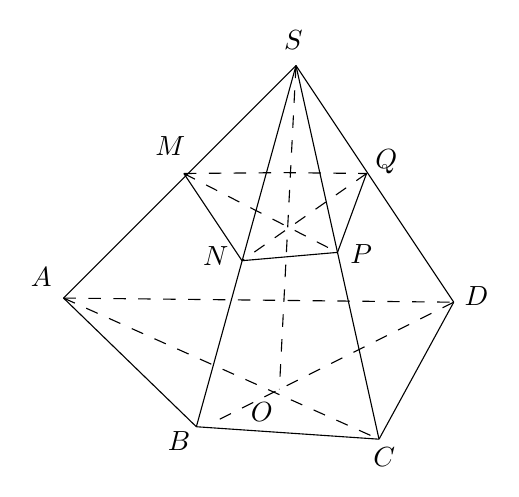
\begin{tikzpicture}[x=0.75pt,y=0.75pt,yscale=-1,xscale=1]
					\draw [dash pattern={on 4.5pt off 4.5pt}]  (140,170) -- (328,172);
					 \draw (140,170) -- (204,232);
					\draw  (292,238) -- (204,232);
					 \draw (328,172) -- (292,238);
					\draw  [dash pattern={on 4.5pt off 4.5pt}] (140,170) -- (292,238);
					\draw [dash pattern={on 4.5pt off 4.5pt}] (328,172)  -- (212,230);
					\draw [dash pattern={on 4.5pt off 4.5pt}]  (252,58) -- (244,214);
					\draw (252,58)  -- (140,170);
					\draw (252,58) --  (204,232);
					\draw (252,58) -- (328,172); 
					\draw (252,58) -- (292,238); 
					\draw (198,110) --  (226,152);
					\draw (286,110) --  (272,148);
					 \draw [dash pattern={on 4.5pt off 4.5pt}] (198,110) -- (245.48,109.57) -- (286,110);
					\draw  (272,148) -- (226,152);
					\draw [dash pattern={on 4.5pt off 4.5pt}] (198,110) -- (272,148); 
					\draw [dash pattern={on 4.5pt  off 4.5pt}] (286,110) -- (226,152);
					\draw (245,40) node [anchor=north west][inner sep=0.75pt] [align=left] {$S$}; 
					\draw (123,154) node [anchor=north west][inner sep=0.75pt] [align=left]  {$A$};
					\draw (189,233) node [anchor=north west][inner sep=0.75pt] [align=left] {$B$}; 
					\draw (288,241) node [anchor=north  west][inner sep=0.75pt] [align=left] {$C$};
					\draw (332,163) node [anchor=north west][inner  sep=0.75pt] [align=left] {$D$};
					\draw  (229,219) node [anchor=north west][inner sep=0.75pt] [align=left] {$O$};
					\draw (183,91) node [anchor=north west][inner sep=0.75pt] [align=left]  {$M$};
					\draw (206,144)  node [anchor=north west][inner sep=0.75pt] [align=left] {$N$};
					\draw  (277,143) node [anchor=north west][inner sep=0.75pt] [align=left] {$P$};
					\draw  (289,97) node [anchor=north west][inner sep=0.75pt] [align=left] {$Q$};
				\end{tikzpicture}
		\end{center}
		 Trong mặt phẳng $ (MNPQ)$ gọi $ I=MP\cap NQ$.\\
		 Ta sẽ chứng minh $ I\in SO$.\\
		Dễ thấy $ S$ là điểm  chung của hai mặt phẳng $ (SAC)$ và $ (SBD)$; đồng thời ta có:\\
		 $\heva{
		 &{O\in AC,AC\subset (SAC)}\\
		&{O\in  BD,BD\subset (SBD)}
		}$ \\$\Rightarrow O\in (SAC)\cap  (SBD).\,$\\
		Vì vậy $  SO=(SAC)\cap (SBD)$.(1)\\
		Mặt khác: $\heva{ 
		&{I\in MP,MP\subset (SAC)}\\ 
		 &{I\in NQ,NQ\subset (SBD).}
		}\Rightarrow I\in  (SAC)\cap (SBD).\,(2)$\\
	 Từ $(1)$ và $(2)$ suy ra $ I\in SO$ hay các đường thẳng $ MP,NQ,SO$ đồng quy tại điểm $ I$.}
\end{ex}

% nguồn: Ok_TraLoiNgan_Lop11_Lan1
\begin{ex}%[1H4V1-6]%[ma:df2cecba]
	 Cho tứ diện $ SABC$. Trên $ SA,SB$ và $ SC$ lần lượt lấy các điểm $ D,E$ và $ F$ sao cho $ DE$ cắt $ AB$ tại $ I,EF$ cắt $ BC$ tại $ J,DF$ cắt $ AC$ tại $ K$. Hỏi ba điểm $ I,J,K$ ở vị trí như thế nào với nhau, nếu thẳng hàng chọn $1$, không thẳng hàng chọn $2$, đồng quy chọn $3$, không nằm ở trường hợp nào của các lựa chọn trước thì chọn $4$.\\
	\shortans{1} 
	 \loigiai{
		Ta chứng minh  ba điểm $ I,J,K$ đều là điểm chung của hai mặt phẳng $ (DEF)$ và $ (ABC)$.\\
		\begin{center}
			\tikzset{every picture/.style={line  width=0.75pt}}
			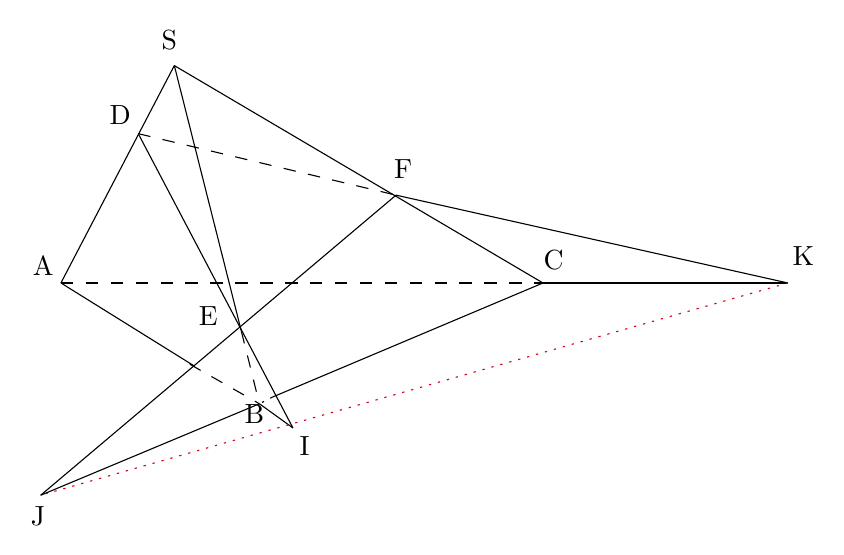
\begin{tikzpicture}[x=0.75pt,y=0.75pt,yscale=-1,xscale=1]
					 \draw [dash pattern={on 4.5pt off 4.5pt}] (183.75,137.74) -- (416.01,137.74);
					 \draw (285.59,192.75) -- (416.01,137.74);
					\draw  (183.75,137.74) -- (248.33,177.94);
					\draw (238.39,33) --  (270.69,161.01);
					\draw  (238.39,33) -- (183.75,137.74);
					\draw  (238.39,33) -- (416.01,137.74);
					\draw [dash pattern={on 4.5pt off  4.5pt}] (221.01,65.8) -- (345.21,95.42);
					\draw (345.21,95.42) --  (534,137.74);
					 \draw (416.01,137.74) -- (534,137.74);
					 \draw (345.21,95.42) -- (174,240);
					\draw (221.01,65.8)  -- (295.53,207.57);
					\draw [dash pattern={on 4.5pt off 4.5pt}]  (245.85,176.88) -- (279.38,195.93);
					 \draw (279.38,195.93) -- (174,240);
					\draw [dash pattern={on 4.5pt off 4.5pt}] (270.69,161.01) --  (279.38,195.93);
					 \draw (295.53,207.57) -- (279.38,195.93);
					\draw [dash pattern={on 0.84pt off 2.51pt}] (285.59,192.75)  -- (279.38,195.93);
					\draw [color={rgb,255:red,208; green,2; blue,27},draw opacity=1] [dash  pattern={on 0.84pt off 2.51pt}] (534,137.74) -- (174,240);
					\draw (231,15)  node [anchor=north west][inner sep=0.75pt] [align=left] {S};
					\draw (169,124) node [anchor=north  west][inner sep=0.75pt] [align=left] {A};
					\draw  (271,195) node [anchor=north west][inner sep=0.75pt] [align=left] {B};
					\draw (249,148) node [anchor=north west][inner  sep=0.75pt] [align=left] {E};
					\draw (343,77) node [anchor=north west][inner sep=0.75pt] [align=left]  {F};
					\draw (535,119) node [anchor=north west][inner sep=0.75pt] [align=left]  {K};
					\draw  (297.53,210.57) node [anchor=north west][inner sep=0.75pt] [align=left] {I};
					\draw (168,244) node [anchor=north west][inner sep=0.75pt] [align=left] {J}; 
					\draw (206,51)  node [anchor=north west][inner sep=0.75pt] [align=left] {D};
					\draw (415,121)  node [anchor=north west][inner sep=0.75pt] [align=left] {C};
				\end{tikzpicture}
		\end{center}
		Ta  có $\heva{
		{I\in DE,DE\subset (DEF)}\\ 
		{I\in AB,AB\subset (ABC).} 
		}$  \\
		$\Rightarrow I\in (DEF)\cap  (ABC).\,(1)$\\
		Tương tự,  ta có $\heva{
		 &{J\in EF,EF\subset (DEF)}\\
		&{J\in  BC,BC\subset (ABC).}
		 }$\\
		$\Rightarrow  J\in (DEF)\cap (ABC).\,(2)$\\
		 $\heva{
		&{K\in  DF,DF\subset (DEF)}\\
		 &{K\in AC,AC\subset (ABC).}
		}$ \\$\Rightarrow  K\in (DEF)\cap (ABC).\, (3)$\\
		Từ $(1)$, $(2)$, $(3)$ suy ra $ I,J,K$ cùng thuộc  hai mặt phẳng $ (DEF),(ABC)$.\\
	Vì vậy ba điểm $ I,J,K$  thẳng hàng.}
\end{ex}

% nguồn: Ok_TraLoiNgan_Lop11_Lan2
\begin{ex}%[1H4V1-6]%[ma:eca99028]
	Cho tứ diện $ABCD$. Gọi $M$,  $P$ lần lượt là trung điểm các cạnh $AD$, $BC$, còn $N$ là điểm trên cạnh $AB$ sao cho $AN=\dfrac{1}{3}AB$. Giao điểm $Q$ của $DC$ với $(MNP)$. Tính tỉ số $\dfrac{DQ}{DC}$ (làm tròn đến hàng phần trăm).
	\shortans{0,33} 
	\loigiai{ 
		\begin{center}
			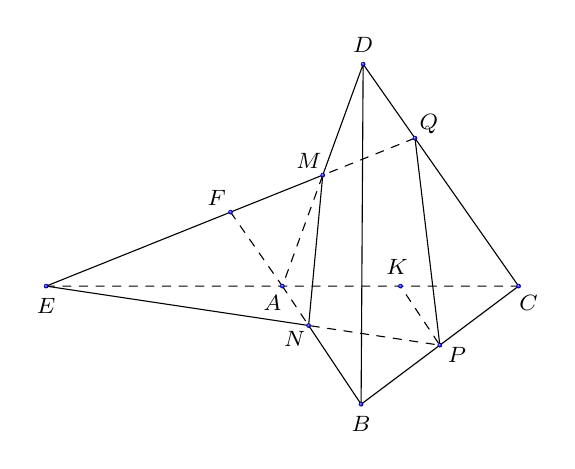
\begin{tikzpicture}[scale=1,>=stealth,font=\footnotesize,line join=round,line cap=round,declare function={h=3;}]
					 \path
						 (0,0) coordinate (A)
						(1,-1.5) coordinate  (B)
						(3,0)  coordinate (C)
						 (A)+(70:h) coordinate (D)
						(barycentric cs:A=1,D=1) coordinate  (M)
						(barycentric cs:B=1,C=1) coordinate (P) 
						(barycentric cs:A=2,B=1)  coordinate (N)
						(intersection of  A--C and N--P) coordinate (E)
						(intersection of E--M and  C--D) coordinate (Q)
						(barycentric  cs:E=1,Q=1) coordinate (F)
						(barycentric cs:A=1,C=1) coordinate  (K);
					 \draw[dashed] (F)--(A)--(M)--(Q)
						 (A)--(N)--(P)--(K)
						(E)--(C); 
					 \draw (D)--(M)--(E)--(N)--(B)--(C)--(D)--(B)
						(M)--(N) 
						(P)--(Q); 
					\foreach  \p/\g in{A/-120,B/-90,C/-60,D/90,M/135,P/-30,Q/45,E/-90,N/-135,F/135,K/100}
					 \shade[shading=ball](\p) circle (.03) node[shift={(\g:.25)},scale=1]{$\p$};
				\end{tikzpicture}
		\end{center}
		Trong  mặt phẳng $(ABC)$, gọi $E=AC\cap NP$.\\
		Ta có $\heva{&(ABC)\cap (MNP)=NP\\  &(ACD)\cap(MNP)=MQ\\ &(ABC)\cap(ACD)=AC\\ &AC\cap NP=E}$ nên ba đường thẳng $NP$, $AC$ và $MQ$ đồng quy tại $E$.\\
		Kẻ $AF\parallel  CD$, $F\in EQ$, kẻ $PK\parallel AN$, $K\in EC$.\\
		Ta có $\dfrac{AF}{DQ}=\dfrac{MA}{MD}=1$ $\Rightarrow$ $AF=DQ$.  \hfill$(1)$\\
		$\dfrac{AF}{QC}=\dfrac{EA}{EC}$. \hfill$(2)$\\ 
		Do $KP=\dfrac{1}{2}AB=\dfrac{1}{2}\cdot 3AN=\dfrac{3}{2}AN$  nên $\dfrac{AN}{KP}=\dfrac{2}{3}$.\\
		 $\dfrac{EA}{EK}=\dfrac{AN}{KP}=\dfrac{2}{3}$ $\Rightarrow$ $\dfrac{EA}{EC}=\dfrac{1}{2}$. \hfill$(3)$\\
		Từ  $(1)$, $(2)$, $(3)$ suy ra $\dfrac{QD}{QC}=\dfrac{FA}{QC}=\dfrac{EA}{EC}=\dfrac{1}{2}$ $\Rightarrow$ $\dfrac{QD}{DC}=\dfrac{1}{3}$.
	 }
\end{ex}


%%%%%%%%%%%%%%%% TỰ LUẬN %%%%%%%%%%%%%%%%

% nguồn: Ok_TuanLuan_Toan11_Lan2
\begin{ex}%[1H4H1-6]%[ma:57fc3e59]
	Cho hình chóp tứ giác $S.ABCD$, gọi $O$ là giao điểm của hai đường chéo $AC$ và $BD$. Một  mặt phẳng $(\alpha)$ cắt các cạnh bên $SA$, $SB$, $SC$, $SD$ tưng ứng tại các điểm $M$, $N$, $P$, $Q$. Chứng minh rằng các đường thẳng $MP$, $NQ$, $SO$ đồng qui.
	 \loigiai{
		\begin{center}
			\begin{tikzpicture}[scale=0.9,font=\footnotesize,line join=round,line cap=round,>=stealth]
					 \path
						(0,0) coordinate  (A)
						(2,-2) coordinate  (B)
						 (4,-1.5) coordinate (C)
						(6,0) coordinate (D) 
						 (3,4) coordinate (S)
						(intersection of A--C and B--D) coordinate  (O)
						($(S)!1/2!(O)$) coordinate (I) 
						($(S)!1/2!(A)$) coordinate  (M)
						($(S)!1/2!(B)$) coordinate  (N)
						($(S)!1/2!(C)$)  coordinate (P)
						($(S)!1/2!(D)$)  coordinate (Q);
					\draw  (C)--(S)--(A)--(B)--(C)--(D)--(S)--(B)
						(M)--(N)--(P)--(Q); 
					\draw[dashed] (D)--(A)--(C) 
						 (B)--(D)
						 (S)--(O)
						(M)--(P) 
						 (N)--(Q)--(M);
					\foreach \p/\g in  {S/135,A/120,B/170,C/-45,D/30,M/125,N/180,P/-45,I/120,O/120,Q/45}
					\fill(\p)  circle (1pt)
						 ($(\p)+(\g:3mm)$) node{$\p$};
				\end{tikzpicture}
		\end{center}
		Trong mặt  phẳng $(MNPQ)$ gọi $I=MP \cap NQ$. Ta sẽ chứng minh $I \in SO$.\\
		Dễ thấy $SO=(SAC) \cap(SBD) \quad  (1)$.\\
		Ta có $\heva{&I \in MP \subset(SAC) \\& I \in NQ \subset(SBD)} \Rightarrow I \in(SAC) \cap (S B  D) \quad (2)$.\\
		Từ $(1)$  và $(2)$ suy ra $ I \in SO$.\\
		Vậy $MP$, $NQ$, $SO$ đồng qui  tại $I$.
	 }
\end{ex}

% nguồn: Ok_TuanLuan_Toan11_Lan2
\begin{ex}%[1H4H1-6]%[ma:2aed9134]
	Cho hình chóp $S.ABC$. Gọi $D$,$E$,$F$ lần lượt là ba điểm trên ba cạnh $SA$, $SB$, $SC$ sao cho $DE$ cắt $AB$  tại $I$,$EF$ cắt $BC$ tại $J$, $FD$ cắt $CA$ tại $K$. Chứng minh ba điểm $I$, $J$, $K$ thẳng hàng.
	\loigiai{ 
		\begin{center}
			\begin{tikzpicture}[scale=1,font=\footnotesize,line join=round,line cap=round,>=stealth]
					\path 
						(0,0) coordinate (A) 
						(1.5,-2) coordinate  (B)
						(5,0)  coordinate (C)
						($(A)+(1,5)$)  coordinate (S)
						($(S)!1/3!(A)$) coordinate (D) 
						($(S)!3/4!(B)$)  coordinate (E)
						($(S)!0.5!(C)$) coordinate  (F)
						(intersection of D--E  and A--B) coordinate (I)
						(intersection of E--F and B--C) coordinate  (J)
						(intersection of F--D  and A--C) coordinate (K)
						(intersection  of E--F and A--B) coordinate (e);
					\draw (S)--(A)--(e) 
						(E)--(S)--(F) 
						(D)--(I) 
						 (F)--(J)
						(F)--(K); 
					 \draw[dashed] (A)--(C)--(B)
						(D)--(F) 
						(C)--(K) 
						(F)--(C) 
						 (B)--(E)
						 (J)--(B)--(I)
						 (B)--(e);
					\draw (J)--(K); 
					\foreach \i/\j in {S/90,A/180,B/-180,C/-45,D/150,E/0,F/45,I/-70,J/-120,K/0}\draw (\i)  circle (1pt) ++(\j:0.3) node {$\i$};
				\end{tikzpicture}
		\end{center}
		Ta có $I=DE \cap AB\Rightarrow  \heva{& I \in DE\subset (DEF) \\&I\in AB\subset (ABC)}\Rightarrow I \in(DEF)\cap \in(ABC).$\\
		Tương tự, ta có $J$,$ K$ cũng thuộc hai mặt phẳng $(DEF)$ và $(ABC)$.\\ 
		Vậy ba điểm $I$, $J$, $K$ thẳng  hàng.
	 }
\end{ex}

% nguồn: Ok_TuanLuan_Toan11_Lan2
\begin{ex}%[1H4H1-6]%[ma:0423144b]
	Cho tứ diện $ABCD$. Gọi $M$, $N$ lần lượt là trung điểm của $AB$ và $CD$.  Mặt phẳng $(\alpha)$ qua $MN$ cắt $AD$, $BC$ lần lượt tại $P$ và $Q$. Biết $MP$ cắt $NQ$ tại $I$. Chứng minh ba điểm $I$, $B$, $D$ thẳng hàng.
	 \loigiai{
		\begin{center}
			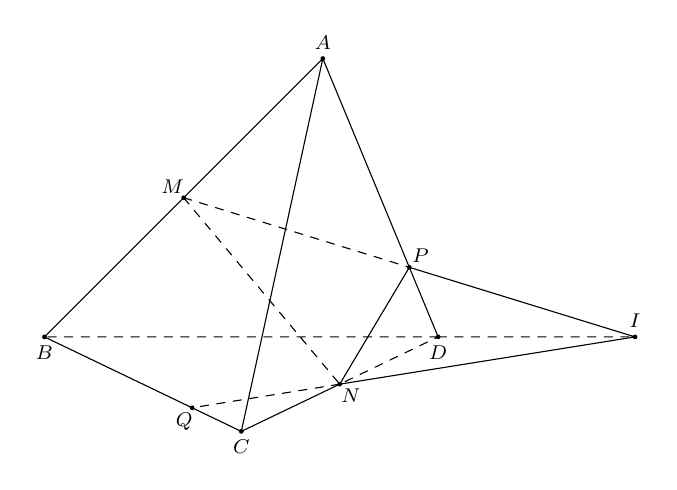
\begin{tikzpicture}[scale=1,>=stealth,font=\footnotesize,line join=round,line cap=round,declare function={h=5;}]
					\path 
						(0,0) coordinate  (B)
						(5,0) coordinate  (D)
						(2.5,-1.2) coordinate (C) 
						(B)+(45:h) coordinate  (A)
						(barycentric cs:B=1,A=1) coordinate  (M)
						(barycentric cs:C=1,D=1) coordinate  (N)
						(barycentric cs:D=3,A=1) coordinate  (P)
						(intersection of M--P and B--D) coordinate (I) 
						(intersection  of N--I and B--C) coordinate (Q);
					\draw[dashed] (D)--(B) 
						 (M)--(P)
						(N)--(Q) 
						 (D)--(I)
						(M)--(N)--(D); 
					 \draw (D)--(A)--(B)--(C)--(N)
						(A)--(C) 
						 (P)--(I)--(N)--(P);
					\foreach \p/\g in {A/90,B/-90,C/-90,D/-90,M/135,N/-45,P/45,I/90,Q/-120}  \fill (\p) circle (.03) node[shift={(\g:.2)},scale=.9]{$\p$};
				\end{tikzpicture}
		\end{center}
		Ta  có $(ABD) \cap(BCD)=BD$.\\
		Lại có $\heva{&I \in MP \subset(ABD) \\& I  \in NQ \subset(BCD)} \Rightarrow I\in (ABD)\cap (BCD)$.\\
		Suy ra $ I  \in BD$. \\
		Vậy ba  điểm $ I$, $B$, $D$ thẳng hàng.
	} 
\end{ex}

% nguồn: Ok_TuanLuan_Toan11_Lan2
\begin{ex}%[1H4H1-6]%[ma:2e124ac5]
	Cho tứ diện $ABCD$. Gọi $E$, $F$, $G$ lần lượt là các điểm  thuộc ba cạnh $AB$, $AC$, $BD$ sao cho $EF$ cắt $BC$ tại $I$, $AD$ cắt $EG$ tại $H$. Chứng minh ba đường thẳng $CD$, $IG$, $HF$ cùng đi qua một điểm.
	\loigiai{ 
		\begin{center}
			\begin{tikzpicture}[scale=0.7]
					 \coordinate [label=left:$B$] (B) at (0,0);
					 \coordinate [label=right:$D$] (D) at (4,-2);
					\coordinate  [label={above,xshift=4pt}:$C$] (C) at (6,0);
					\coordinate [label=above:$A$]  (A) at (2,5);
					\coordinate [label=left:$E$] (E) at  ($(A)!1/2!(B)$);
					\coordinate [label=below:$H$] (H) at  ($(A)!1.5!(D)$);
					\coordinate [label=right:$I$] (I) at  ($(B)!1.5!(C)$);
					\path [name path=AC] (A)--(C); \path [name  path=EI] (E)--(I);
					\path [name intersections={of=AC and EI,by={[label=above right:$F$]F}}]; 
					\path [name path=BD] (B)--(D); \path [name path=EH]  (E)--(H);
					\path [name intersections={of=BD  and EH,by={[label= below left:$G$]G}}];
					\path [name path=CD] (C)--(D); \path  [name path=GI] (G)--(I);
					\path [name intersections={of=CD and GI,by={[label=below  right:$O$]O}}];
					\foreach \point in {A,B,C,D,E,F,H,I,G,O} \fill  (\point) circle (1pt);
					\draw[dashed]  (B)--(I)
						 (E)--(F)
						(G)--(O)--(C)--(F); 
					\draw (A)--(B)--(D)--(O)--(A) 
						 (O)--(I)
						 (F)--(I)
						 (E)--(H)--(F)
						 (A)--(F)
						 (A)--(H);
				\end{tikzpicture}
		\end{center}
		Gọi $O=HF \cap IG$.\\ 
		Suy ra $\heva{&O  \in HF\subset(ACD)\\& O\in IG\subset(BCD)}\Rightarrow O \in(ACD) \cap(BC D) \quad (1)$.\\
		Mặt khác, ta  có $(ACD) \cap(BCD)=CD \quad (2)$.\\
		 Từ $(1)$ và $(2)$, suy ra $O \in CD$.\\
		Vậy ba đường thẳng  $CD$, $IG$, $HF$ cùng đi qua một điểm.
	 }
\end{ex}

% nguồn: Ok_TuanLuan_Toan11_Lan1
\begin{bt}%[1H4V1-6]%[ma:d20be1fb]
	Cho tứ diện $ ABCD$. Gọi $ E,F,G$ là các điểm lần lượt thuộc các cạnh $ AB,AC,BD$ sao cho $ EF$ cắt $ BC$ tại $ I,EG$ cắt $ AD$ tại $ H$. Nếu ba đường thẳng $ CD, IG, HF$  đồng quy thì chọn $1$, không đồng quy thì chọn $2$, song song thì chọn $3$, chéo nhau thì chọn $4$, không nằm ở trường hợp nào của các lựa chọn trước thì chọn $5$.
	 \loigiai{
		Trong mặt phẳng  $ (BCD)$, gọi $ O=CD\cap IG$.\\
		Ta có $\heva{ 
		 &{O\in IG,IG\subset (EFH)}\\
		&{O\in  CD,CD\subset (ACD)}
		}$  \\
		$\Rightarrow O\in (EFH)\cap  (ACD).\,(1)$\\
		Mặt khác: $ H\in AD,AD\subset (ACD)\Rightarrow H\in (ACD)\Rightarrow  H\in (ACD)\cap (EFH)$.\\
		Tương  tự: $ F\in AC,AC\subset (ACD)\Rightarrow F\in (ACD)\Rightarrow F\in (ACD)\cap (EFH)$.\\
		Vì vậy  $ HF=(ACD)\cap (EFH).\, (2)$\\
		Từ $(1)$ và $(2)$ suy ra $O$ thuộc $ HF$ hay  $ CD,IG,HF$ đồng quy tại $ O$.\\
	 }
\end{bt}

% nguồn: Ok_TuanLuan_Toan11_Lan2
\begin{ex}%[1H4V1-6]%[ma:b477ddd2]
	Cho tứ diện $ ABCD$. Gọi $ E,F,G$ là các điểm lần lượt thuộc các cạnh $ AB,AC,BD$ sao cho $ EF$ cắt $ BC$ tại $ I,EG$ cắt $ AD$ tại $ H$. Nếu ba đường thẳng $ CD, IG, HF$ đồng quy thì chọn $1$, không đồng quy thì chọn $2$, song song thì chọn $3$, chéo nhau thì chọn $4$, không nằm ở trường hợp nào của các lựa chọn trước thì chọn  $5$.
	 \loigiai{
		Trong mặt phẳng $ (BCD)$, gọi $ O=CD\cap  IG$.\\
		Ta có $\heva{ 
		 &{O\in IG,IG\subset (EFH)}\\
		&{O\in  CD,CD\subset (ACD)}
		}$ \\ 
		$\Rightarrow O\in (EFH)\cap (ACD).\,(1)$\\ 
		Mặt khác: $ H\in AD,AD\subset  (ACD)\Rightarrow H\in (ACD)\Rightarrow H\in (ACD)\cap (EFH)$.\\
		Tương tự: $ F\in AC,AC\subset (ACD)\Rightarrow F\in (ACD)\Rightarrow F\in (ACD)\cap (EFH)$.\\ 
		Vì  vậy $ HF=(ACD)\cap (EFH).\, (2)$\\
		Từ  $(1)$ và $(2)$ suy ra $O$ thuộc $ HF$ hay $ CD,IG,HF$ đồng quy tại $ O$.\\
	 }
\end{ex}
